\begin{figure}[h!tb]
\centering
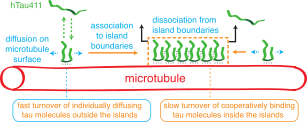
\includegraphics[width=0.6\textwidth]{Figures/tau8.png}
\caption[Schematic representation of island formation.]{
\textbf{Schematic representation of island formation.} Tau molecules bind and unbind with high rates to microtubules, on which they diffuse (fast turnover). When encountering an island (dashed orange box), tau molecules cooperatively associate with the island at its boundaries, rendering the tau molecules stationary, decreasing their unbinding rate (slow turnover), and causing the island to grow in size laterally. Tau molecules from solution can only bind to the inside of an island via displacement of an island-associated tau molecule, resulting in the observed concentration-dependent turnover of tau inside islands. After removal of tau from solution, tau molecules dissociate from the island boundaries, making the island shrink in size laterally.
	}\label{tau8}
\end{figure}
In our investigation of tau interactions with microtubules, we have contributed to our understanding of the distinct binding modes of tau to the microtubule, thereby contributing to our understanding of potential molecular mechanisms governing axonal microtubule arrays. While the diffusive binding mode of tau to mts was already well-described, our key contribution is that tau can cooperatively bind to form cohesive islands on the microtubule. Our findings, coupled with complementary work by \cite{tan2019microtubules}, paint a detailed picture of tau's multifaceted behavior on microtubules.\par

The cooperative binding mode results in a population of stationary tau molecules characterized by remarkably low turnover rates. This is in contrast to the diffusive mode, where tau molecules exhibit high turnover rates. At physiological concentrations, these two distinct populations coexist on the microtubule surface. It is possible that these islands have not yet been described is because the rapidly turning over tau has the potential to mask the underlying island structures, adding a layer of complexity to the visualization and study of these formations \aref{tau8}{}. It is also possible that \cite{Mcvicker2014} had already observed the cooperative binding mode underlying the formation of tau islands, given that they describe the association of a small number of tau molecules and a concomitant marked reduction of the diffusion coefficient of tau. This view is supported by their observation that these small tau complexes only formed on paclitaxel-stabilized microtubules, but not on GMPCPP-stabilized mts, which aligns with the same observations by \cite{tan2019microtubules} regarding the formation of tau islands. That \cite{Mcvicker2014} did not observe "fully formed" islands could potentially be explained by different assay conditions, e.g., the use of a different buffer. Also, \cite{Mcvicker2014} used a lower tau concentration (5nM). In case of the condition at which they did use a high concentration (300nM), most of the tau was not labeled, hence it is possible that islands were present in the assay but not visible.\par

We measured a characteristic density within tau islands of approximately 0.26 tau molecules per tubulin dimer. This value would indicate the formation of an ordered monolayer, likely involving all four microtubule-binding repeats of tau, as suggested by the cryo-EM study by \cite{Kellogg2018} (see \aref{sec:tau_intro}{}). It bears noting that the diffusive, rapidly turning over tau population likely is too elusive to detect in these structural studies due to its transient and fast-moving nature. In addition, this type of binding may reflect the intrinsically disordered nature of tau, and thus not result in any favored binding conformations where an averaging of multiple binding events would lead to an increase in resolution.\par 

The integrity of tau islands appears to hinge on cooperative interactions between the constituent molecules. This cooperativity could stem from direct tau-tau interactions, a hypothesis supported by previous studies demonstrating tau's propensity for liquid-liquid phase separation \parencite{HERNANDEZVEGA20172304} and its ability to form neurofibrillary tangles when hyperphosphorylated \parencite{iqbal2016tau}. Alternatively, or perhaps additionally, this cooperativity might arise from local tau-induced impacts on the microtubule lattice. Such modifications could conceivably translate along the microtubule lattice to adjacent binding sites, thereby enhancing the affinity for incoming tau molecules. This possibility is supported by two observations: 
\begin{enumerate}
    \item Within regions of high microtubule curvature, in contrast to surrounding regions, we observed tau binding to persist after tau had been removed from solution, a characteristic it shared with tau molecules within tau islands.
    \item \cite{tan2019microtubules} had reported that islands did not grow on GMPCPP-stabilized microtubules. GMPCPP lattices feature a higher axial repeat, in other words, an expanded lattice when compared to paclitaxel-stabilized mts \pref{sec:stabilization}{}.
\end{enumerate}
I had thus hypothesized that tau islands may require a specific spacing of tubulin dimers to accommodate a proper binding of all microtubule binding repeats. This spacing, I hypothesized, was given both in the case of high-curvature regions as well as within island regions (on paclitaxel-stabilized mts). 
\begin{itemize}
    \item In the case of islands, a favorable MT region would at first allow for island nucleation, upon which these initial tau molecules would change the spacing of tubulin dimers in their vicinity, allowing for additional tau molecules to bind, leading to island growth.
    \item  In the case of high-curvature regions, it is clear that the tubulin dimers are spaced differently than on straightd microtubule regions. In the inside of the curved region, tubulin dimers are closer to each other, while on the outside, dimers are further apart from each other. Thus, if the stationary tau binding mode indeed possesses a preference for a different lattice spacing than given on a (undecorated) straight microtubule, it appears likely that this binding mode does occur on some parts of curved microtubules (likely on the inside, given that the non-binding to GMPCPP lattices indicates a preferences for compacted lattices). Importantly, this type of stationary binding would not require any cooperative behavior, and would even preclude such cooperative binding and its concomitant shielding of the microtubule from katanin severing, as we had observed, see e.g. \aref{taucurve}{F-H} (given mechanical constraints set by the microtubule and the antibodies it is bound to, though we did frequently observe tau islands to straighten curved microtubule regions). 
\end{itemize}
Indeed, this hypothesis was confirmed in a follow-up study by my former colleague Valerie Siahaan and collaborators: They found that the cooperative tau binding mode of tau depends on and stabilizes a compacted microtubule lattice \parencite{siahaan2022microtubule}. As a small deviation from my initial reasoning above, while the slightly lower axial repeat of paclitaxel-stabilized mts as compared to GMPCPP-stabilized mts may facilitate initial binding, the main reason for why islands can form on paclitaxel-stabilized mts appears to be that cooperative tau binding displaces paclitaxel from its binding site, further compacting the lattice to an axial repeat similar to that of unstabilized GDP lattices \parencite{siahaan2022microtubule}. Indeed, \cite{siahaan2022microtubule} found tau to readily bind cooperatively to unstabilized GDP lattices, and the introduction of paclitaxel to cause the destabilization of tau islands and tau unbinding.\par

Given that some MAPs are known to affect the spacing of tubulin dimers, one is tempted to ask whether regulation of the microtubule axial repeat is a common feature of MAP regulation. For example, kinesin-1 is known to expand the microtubule lattice \pcite{Peet2018}, which could explain why it does not bind to island regions as shown by Valerie's work for our article showed cannot enter tau islands (and the associated compacted mt lattice) \pcite{Siahaan2019a}. Thus, \cite{siahaan2022microtubule} have also investigated whether the other members of the tau/MAP2/MAP4 family bind cooperatively to the lattice. They found that while MAP4 does not form islands, MAP2 does, and that MAP2 can form islands together with tau (while MAP4 does not partition into these islands). The indirect interplay of different MAPs on microtubules via changes of the microtubule lattice could add another dimension to MAP sorting and regulation. For example, MAP7 and tau exclude each other when binding to the microtubule, and, oppositely to tau, MAP7 recruits kinesin-1 binding to the microtubule \cite{Monroy2018}, which could point to such an indirect lattice-based interplay. It is conceivable that the displacement of tau by kinesin-8/Kip3 could also constitute an instance of such an interplay: Given that kinesin-1 has been found to expand the microtubule lattice, it appears possible that kinesin-8 may also cause lattice expansion, thereby causing the disassembly of tau islands. However, a point against such a hypothesis is the fact that Kip3 has been observed to have a higher affinity for taxol-stabilized microtubules than for GMPCPP-stabilized microtubules \pcite{Hugo}, which is the opposite of what has been observed for kinesin-1 \pcite{Nakata2011}. Importantly, this could explain our finding that Kip3 can penetrate tau islands while kinesin-1 cannot.\par

It also is tempting to speculate that the absence of tau from highly curved microtubules \textit{in vivo} may fulfill a regulatory purpose by allowing for a katanin-mediated removal of ill-positioned microtubules. In this respect, it should be noted that another MAP, doublecortin, has already been shown to both bind to microtubules cooperatively and bind to curved microtubule regions as well \parencite{Bechstedt2012, Bechstedt2014}. \cite{Bechstedt2012} had also found doublecortin to be sensitive to the number of protofilaments of a given microtubule, in particular, it appeared to stabilize 13-protofilament microtubules. Interestingly, in a different study, tau had also been found to be sensitive to protofilament number, apparently stabilizing 14-protofilament microtubules \pcite{Choi2009}. Indeed, 14-protofilament-microtubules were the most common mt population in the study by \cite{Kellogg2018}. These similarities of tau are particularly notable as doublecortin does not share any sequence homology with tau, and in particular it appears to be more ordered, with its two repeat domains forming globular structures \pcite{Moores2004}. A better comparative understanding of the features of tau and doublecortin may be insightful for exploring the mechanisms underlying these features. Moreover, both doublecortin and tau are located in neurons, and in contrast to MAP2, doublecortin does not share a binding site with tau \pcite{Moores2004}. Thus, it would be interesting to explore the potential interplay of these MAPs on the microtubule surface \textit{in vitro}, which to my knowledge has not yet been done. \par

Another intriguing observation from our study was that tau unbinding from islands increases with rising tau concentration in solution. Importantly, this phenomenon cannot be attributed solely to the rapidly turning over tau pool that co-localizes with islands at elevated concentrations. At 20 nM and 100 nM tau, this pool accounts for only approximately 20\% and 40\% of the total tau in the islands, respectively, while the average unbinding time drops by two orders of magnitude. We propose that this concentration-dependent unbinding results from the multivalent attachment of island-incorporated tau, mediated by its four microtubule-binding repeats and potential tau-tau interaction sites. Such concentration-dependent unbinding mechanism has been previously reported for other multivalently interacting macromolecules, in the case of microtubules as well as DNA \parencite{lanskydiffusible2015, sing2014multiple}. Specifically, our model suggests that the multiple interaction sites undergo transient cycles of unbinding and rebinding. At low tau concentrations, transiently released bonds are likely reestablished as partially-bound tau molecules remain anchored to the microtubule by their persisting binding sites. However, with increasing tau concentration in solution, it becomes increasingly probable that a binding site of a solution-phase tau molecule establishes a bond to a temporarily-vacated binding site on the microtubule. This process could sequentially replace an island-incorporated tau molecule, one bond at a time. Similarly, a step-by-step displacement mechanism could also be at play in the case of kinesin-8-driven island disassembly.

Beside probing the mechanisms behind the displacement of tau islands by Kip3, our results further suggest an intriguing avenue for further research in this respect. For example, one can envision cycles of island growth, kinesin-8 traffic jam formation at island boundaries, eventual overwhelming and disassembly of the island by Kip3, propagation of the traffic jam as a high-density "pulse" along the microtubule, followed by island regrowth and repetition of the process. This dynamic interplay could potentially result in pulsatile kinesin-8 movement along axonal microtubules, adding another layer of complexity to cellular transport regulation.\par


All of the above points, the consistent density of islands, of 0.26 tau molecules per tubulin dimer, the (now-confirmed) dependence of the cooperative binding mode on a specific lattice constant \parencite{siahaan2022microtubule} as well as the concentration-dependence of tau unbinding from island regions hint at an integral role of the microtubule binding repeats in the cooperative binding mode. Our (not-yet-published) findings regarding the ionic strength dependence of island stability \pref{tausalt}{} provide further support for the involvement of microtubule binding repeats in cooperative binding. We observed optimal stability at 75mM KCl, suggesting a delicate balance between hydrophobic interactions, likely mediated by the repeats, and ionic interactions, potentially mediated by the more positively-charged C-terminal domain of tau. The stronger diffusive mode at 0mM KCl indeed implies a predominance of ionic bonds in this binding mode and is consistent with the findings of \cite{Hinrichs2012b} who found the tau diffusion coefficient to decrease with decreasing ionic strength. These ionic strength dependencies could also explain the varying stationarity of tau molecules within islands at different KCl concentrations. At lower KCl concentrations, single tau molecules within islands were less stationarily bound, potentially switching binding modes more frequently and often having only a subset of their microtubule binding repeats engaged.\par

Our findings can also be interpreted as supporting the feasibility of the polymer brush model of microtubule spacing in axonal microtubule arrays. As mentioned in \aref{sec:tau}{}, the N-terminal domain of tau determines the spacing between axonal microtubules. The argument by \cite{Gaspard} against the polymer brush model was that the stoichiometry of tau:tubulin in the axon is likely too low for tau-decorated microtubules to be repelled from each other, as tau molecules can simply diffuse away from the inter-microtubule space, is weakened due to points:
\begin{enumerate}
    \item Our study supports the model that one (full-length) tau molecules binds 4 tubulin dimers, which reduces the required number of tau molecules to fully cover the microtubule compared to models where tau binds to e.g. only 1 tubulin dimer.
    \item Moreover, within tau islands, diffusion is greatly reduced, thus it is thinkable that tau islands interspersed on a given microtubule would be sufficient to keep microtubules apart, i.e. full coverage of the microtubule would not be possible. Curiously, a recent study employing super-resolution fluorescence imaging combined with antibody-based fluorescent labeling of all tau isoforms reported that within rat neurons, tau forms complexes interspersed on the microtubule \pcite{Gyparaki2021}. These complexes in my view could potentially be tau islands.
\end{enumerate}

It bears noting that the model of 4-repeat binding of full-length tau to the microtubule as supported by \cite{Kellogg2018} and our findings is in conflict with the model proposed by \cite{Mammeri}. This is chiefly because the model proposed by \cite{Mammeri} would suggest each tau molecule to bind only one tubulin dimer tightly. This binding is proposed to take place via the highly positively charged pseudorepeat R' and repeat R4, while the remaining repeats to progressively detach from the microtubule. It is important to note that this proposed binding mode would also constitute longitudinal binding to protofilaments and feature interactions with multiple tubulin dimers. Thus, it would not be incompatible with our proposed mechanism for concentration-dependent unbinding. Furthermore, the finding by \cite{Mammeri} that tau binding is more unstable on GMPCPP-stabilized microtubules than on paclitaxel-stabilized mts appears consistent with our findings. However, the fact that the NMR spectra observed by \cite{Mammeri} did not differ significantly when cutting off the N-terminal domain of tau (which we observed to be necessary for island formation) raises the possibility that their experimental conditions did not precipitate tau island formation.\par

Finally, the comparatively high tau island nucleation rate right after flushing in tau \pref{tauGROW}{G} implies that some microtubule regions are more suitable for the nucleation of tau islands than others. This could be due to mechanical constraints related for instance to where a given microtubule is tied to the coverslip surface via an antibody. Another determinant of island growth could be post-translational tubulin modifications. Indeed, recent \textit{in vitro} experiments have shown that polyglutamylation of tubulin results in a higher affinity of tau for microtubules and a higher rate of island formation \pcite{Genova2023}. Thus, tau island formation may potentially serve as a readout of such modifications, which would in effect allow to amplify the impact of such modifications given the distinct and striking interaction patterns of tau islands with other MAPs. Vice versa, modifications of tau could impact its ability to form islands. Indeed, the data presented in a recent preprint suggests that hyperphosphorylation of tau negatively affects island integrity, decreasing their protection against severing by Katanin \pcite{Siahaan2024}. One may wonder about the significance of these findings for the neuronal context, which is why it is notable that \cite{siahaan2022microtubule} had cultured cells with tau fused to GFP, and upon introducing paclitaxel, had observed an unbinding of tau conspicuously similar to the disassembly of tau islands as we had reported in \aref{tauSHRINK}{}. This strongly indicates that tau islands indeed are a biologically relevant phenomenon. The implications of the findings presented in this thesis and in the work building on it thus extend to neurodegenerative diseases, where alterations in tau's ability to form islands could trigger various downstream pathophysiological effects.